%\newcommand{\ein}[2]{(#1) (#2 Punkte)}


\begin{Large}
\textbf{Teil I: Offene Fragen (38 Punkte)}
\end{Large}
\\
\\
\\
\textbf{Allgemeine Anweisungen für offene Fragen:}
\\
\renewcommand{\labelenumi}{(\roman{enumi})}
\begin{enumerate}
\item
Ihre Antworten müssen alle Rechenschritte enthalten,
diese müssen klar ersichtlich sein.
Verwendung korrekter mathematischer Notation wird erwartet
und fliesst in die Bewertung ein.

\item
Ihre Antworten zu den jeweiligen Teilaufgaben müssen in den dafür vorgesehenen Platz geschrie-
ben werden. Sollte dieser Platz nicht ausreichen, setzen Sie Ihre Antwort auf der Rückseite oder
dem separat zur Verfügung gestellten Papier fort. Verweisen Sie in solchen Fällen ausdrücklich
auf Ihre Fortsetzung. Bitte schreiben Sie zudem Ihren Vor- und Nachnamen auf jeden separaten
Lösungsbogen.

\item
Es werden nur Antworten im dafür vorgesehenen Platz bewertet. Antworten auf der Rückseite
oder separatem Papier werden nur bei einem vorhandenen und klaren Verweis darauf bewertet.

\item
Die Teilaufgaben werden mit den jeweils oben auf der Seite angegebenen Punkten bewertet.

\item
Ihre endgültige Lösung jeder Teilaufgabe darf nur eine einzige Version enthalten.

\item
Zwischenrechnungen und Notizen müssen auf einem getrennten Blatt gemacht werden. Diese
Blätter müssen, deutlich als Entwurf gekennzeichnet, ebenfalls abgegeben werden.
\end{enumerate}

\newpage
\section*{\hfil Aufgaben \hfil}
\vspace{1cm}
\section*{Aufgabe 1 (38 Punkte)}
\vspace{0.4cm}
%\titleformat{\subsection}[runin]
%{\normalfont\large\bfseries}{\thesubsection}{1em}{}
\subsection*{\aufgabe{a1}{8}} 
Die Wirtschaftsredakteurin eines wichtigen Verlagshauses zieht in Betracht,
kostenlose Exemplare eines Buchs an Dozierende der Wirtschaftswissenschaften an Schweizer Hochschulen zu verschicken, da sie weiss, dass Dozierende dazu neigen, Bücher als Kurslektüre auszuwählen, die sie bereits in ihren Regalen stehen haben. Die Fixkosten dieser Werbekampagne belaufen sich auf $100'000$ Schweizer Franken.
Die Stückkosten eines einzelnen Buchs betragen $10$ Schweizer Franken, im Handel werden die Bücher schließlich für $40$ Schweizer Franken pro Exemplar verkauft.
Auf der Basis historischer Daten schätzt die Redakteurin, dass wenn $x$ Gratisexemplare versendet werden, ein Verkauf von insgesamt
\begin{align*}
	B(x) = 20'000 - 19'000 e^{-0.0002 x }
\end{align*}
Exemplaren des Buchs erzielt wird. \\
\\
Zeigen Sie, dass wenn die Produktion auf maximal $6'000$ Bücher beschränkt ist, es genau eine Menge $ x^\star \in (0, 6'000)$ an Gratisexemplaren gibt, bei der die Gesamtkosten genau durch den Umsatz gedeckt werden.


\subsection*{\aufgabe{a2}{8}}
Die Wirtschaftsredakteurin eines wichtigen Verlagshauses zieht in Betracht,
kostenlose Exemplare eines Buchs an Dozierende der Wirtschaftswissenschaften an Schweizer Hochschulen zu verschicken, da sie weiss, dass Dozierende dazu neigen, Bücher als Kurslektüre auszuwählen, die sie bereits in ihren Regalen stehen haben. Die Fixkosten dieser Werbekampagne belaufen sich auf $100'000$ Schweizer Franken.
Die Stückkosten eines einzelnen Buchs betragen $10$ Schweizer Franken, im Handel werden die Bücher schließlich für $40$ Schweizer Franken pro Exemplar verkauft.
Auf der Basis historischer Daten schätzt die Redakteurin, dass wenn $x$ Gratisexemplare versendet werden, ein Verkauf von insgesamt
\begin{align*}
	B(x) = 20'000 - 19'000 e^{-0.0002 x }
\end{align*}
Exemplaren des Buchs erzielt wird. Wenn die Produktion auf maximal $6'000$ Bücher beschränkt ist, gibt es genau eine Menge $ x^\star \in (0, 6'000)$ an Gratisexemplaren, bei der die Gesamtkosten genau durch den Umsatz gedeckt werden.\\
\\
Verwenden Sie eine Taylor-Approximation zweiter Ordnung im Punkt $x_0 = 750$, um eine Näherung für $x^\star$ zu finden.
 \\
\\

\subsection*{\aufgabe{b}{12}}
Anne und Robert haben gerade erfolgreich ihr Masterprogramm in Quantitativen
Methoden an der Universität St.Gallen abgeschlossen und sind nun dabei, ihre eigene
Firma AlgoTrade aufzubauen, die Machine Learning Algorithmen für den computergesteuerten Handel an Finanzmärkten entwickelt. Sie haben bereits viele vielversprechende Ideen, jedoch fehlt ihnen das Eigenkapital. Die anfänglichen Investitionen für den Kauf der IT-Infrastruktur und für die Entwicklung der Software belaufen sich auf $1'500'000$ Schweizer Franken.
Ein Risikokapitalgeber ist zu einem Investment in Höhe von $500'000$ Schweizer Franken bereit, verlangt aber im Gegenzug einen Anteil von $30 \%$ an der Firma.
Zusätzlich nehmen Anne und Robert am 1. Januar 2022 einen Kredit in Höhe von $1'000'000$ Schweizer Franken zu einem jährlichen Zinssatz von $2 \% $ auf.
Die Bank verlangt dabei, dass $40 \%$ des geschuldeten Betrags bis Ende 2026 über konstante Zahlungen $C$, fällig jeweils am Jahresende, zurückgezahlt sein muss.
\begin{enumerate}
	\item[(b1)] Fügen Sie die Ereignisse und Mittelflüsse dem Zeitstrahl hinzu.
	\item[(b2)] Berechnen Sie die Höhe der Ratenzahlung $C$.
\end{enumerate}
Bereits nach 3 Jahren ist AlgoTrade sehr erfolgreich und generiert beträchtliche Umsätze. Beginnend mit der nächsten Rückzahlung am 31. Dezember 2025 wollen Anne und Robert jeweils $180'000$ Schweizer Franken am Ende jedes Jahres solange zurückzahlen, bis die bestehende Restschuld komplett getilgt ist.
\begin{enumerate}
	\item[(b3)] Ergänzen Sie die Information am Zeitstrahl und berechnen Sie die Restschuld am 1. Januar 2025, also direkt nach der jüngsten Rückzahlung.
	\item[(b4)] Am 1. Januar 2029, direkt nach der jüngsten Rückzahlung, verkaufen Anne und Robert	ihre Firma für $5'000'000$ Schweizer Franken und tilgen mit ihrem Anteil die bestehende	Restschuld. Wie hoch ist ihr Gewinn?
\end{enumerate}
\begin{center}
	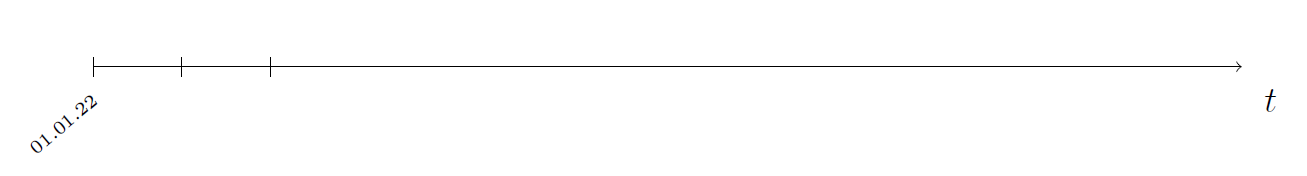
\includegraphics[scale=0.45]{pictures/zeitstrahl_1_b}
\end{center}
\newpage
\subsection*{\aufgabe{c}{10}}
Information spielt in der Entscheidungsfindung eine wesentliche Rolle. Allerdings
sehen sich Unternehmen, wie wir erst kürzlich beobachten konnten, einem Zielkonflikt
ausgesetzt. Einerseits ermöglicht das Sammeln möglichst genauer privater Informationen eine verbesserte, massgeschneiderte Lösung für ihre Kunden (die zu einem höheren Preis verkauft werden kann), andererseits erhöht es den potentiellen Schaden, den sie ihren Kunden durch Datenschutzverletzungen (und sich selbst durch mögliche juristische Folgen) zufügen könnten.\\
\\
Sei $I \geq 0 $ die Menge an Informationen, die ein Unternehmen sammelt, und $b(I)$ der Nutzen für den Kunden hinsichtlich der angebotenen Dienstleistung oder des angebotenen Produktes. Wir nehmen an, dass:
\begin{align*}
	b(I)
	= 
	\begin{cases}
		0 &\quad \textrm{für } 0 \leq I  < I_0\\
		s \left( 1 - \frac{I_0}{I} \right) & \quad \textrm{für } I \geq I_0
	\end{cases}.
\end{align*}
Demnach ist $I_0 > 0 $ die Mindestmenge an Information, die benötigt wird, um einen Nutzen für den Kunden zu generieren, und der Nutzen ist durch $s > 0 $ beschränkt, d.h., der Nutzen wird nie grösser als $s$, egal wie viel Information gesammelt wird. Im Gegensatz dazu soll der erwartete Schaden durch eine Datenschutzverletzung durch
\begin{align*}
	d(I) = \frac{1}{2} q s I^2
\end{align*}
gegeben sein, wobei $q \in (0,1)$ die Wahrscheinlichkeit einer solchen Verletzung darstellt.
Zudem nehmen wir an, dass $q I_0^2 < \frac{8}{27}$ gilt. Für einen potentiellen Kunden ist die relevante Grösse der Trade-off $v(I)$ zwischen dem Nutzen $b(I)$ und dem möglichen Schaden $d(I)$, d.h., $v(I) = b(I) - d(I)$.\\
\\
Für welche Menge $I^\star \geq 0$ an Informationen erzielt der Kunde den bestmögliche Trade-off, d.h. den grössten Wert für $v$?
Bestimmen Sie die Antwort in Abhängigkeit der Parameter $s, I_0, q$.
Weisen Sie nach, dass $I^\star$ tatsächlich ein Maximum von $v$ ist.\\
\\
\textit{Hinweis:} Die Bedingung $q I_0^2 < \frac{8}{27}$ stellt sicher, dass $I^\star > I_0 $ gilt.

\newpage


\fancyhead[C]{\normalsize\textbf{$\qquad$ Teil II: Multiple-Choice}}
\begin{Large}
\textbf{Teil II: Multiple-Choice-Fragen (62 Punkte)}
\end{Large}
\\
\\
\\
\textbf{Allgemeine Anweisungen für Multiple-Choice-Fragen:}
\\
\renewcommand{\labelenumi}{(\roman{enumi})}
\begin{enumerate}
\item
Die Antworten auf die Multiple-Choice-Fragen müssen im dafür vorgesehenen Antwortbogen ein-
getragen werden. Es werden ausschliesslich Antworten auf diesem Antwortbogen bewertet. Der
Platz unter den Fragen ist nur für Notizen vorgesehen und wird nicht korrigiert.

\item
Jede Frage hat nur eine richtige Antwort. Es muss also auch jeweils nur eine Antwort angekreuzt werden.

\item
Falls mehrere Antworten angekreuzt sind, wird die Antwort mit 0 Punkten bewertet, auch wenn
die korrekte Antwort unter den angekreuzten ist.

\item
Bitte lesen Sie die Fragen und die Anweisungen sorgfältig.

\end{enumerate}
\newpage
\section*{Aufgabe 2 (34 Punkte)}
\vspace{0.4cm}

\subsection*{\frage{1}{3}}
$ A $ und $ B $ seien zwei Aussagen. Welche der folgenden zwei zusammengesetzten Aussagen sind äquivalent? 
 \renewcommand{\labelenumi}{(\alph{enumi})}
\begin{enumerate}
\item $ A \Rightarrow   \neg B $ und $\neg (A \wedge B)$.
\item $ A \wedge B $ und $\neg (A \wedge B)$.
\item $ (A \Rightarrow \neg B) $ und $A \wedge B$
\item Keine der obigen Antworten ist richtig.
\end{enumerate}
\ \\
\subsection*{\frage{2}{4}}
Welche der folgenden zusammengesetzten Aussagen ist \textit{keine} Tautologie? 
\renewcommand{\labelenumi}{(\alph{enumi})}
\begin{enumerate}
	\item $( \neg A \vee \neg B ) \Leftrightarrow (\neg  (A \wedge B))$.
	\item $ A \Rightarrow ( B \Rightarrow A)$.
	\item $ ((A \Rightarrow B) \wedge \neg  B) \Rightarrow \neg A$
	\item $ \neg ( \neg A \wedge \neg  B ) \vee B$.
\end{enumerate}
\ \\
\subsection*{\frage{3}{4}}
Seien $\{a_k\}_{k \in \mathbb{N}}$ und $\{b_k\}_{k \in \mathbb{N}}$ zwei geometrische Folgen mit $a_1 = 1$, $a_2= 1.05$ und $b_1 = 2$, $b_2 = 1.9$. Seien $\{s_n^a \}_{n \in \mathbb{N}}$ und $\{s_n^b \}_{n \in \mathbb{N}}$ die entsprechenden Reihen.\\
\\
Welche der folgenden Aussagen ist korrekt?
\renewcommand{\labelenumi}{(\alph{enumi})}
\begin{enumerate}
\item 
Es gibt genau ein $n^\star \in \N$, sodass $s^b_{n^\star} = s^a_{n^\star} $.
\item 
Es gibt genau ein $n^\star \in \N$, sodass $s^b_n \geq s_n^a$ für alle $n \geq n^\star$ und $s_n^b < s_n^a$ für alle $n < n^\star$.
\item 
 $s_n^b < s_n^a$ für alle $n \in \N$.
\item
Es gibt genau ein $n^\star \in \N$, sodass $s_n^b \geq s_n^a$ für alle $n \leq n^\star$ und $s_n^b < s_n^a$ für alle $n > n^\star$.
\item 
$s_n^b > s_n^a$ für alle $n \in \N$.
\end{enumerate}
\ \\
\subsection*{\frage{4}{3}}
Bei einer stetigen Verzinsung mit jährlichem Zinssatz $i$ ist der effektive Jahreszins $i_{\mathrm{eff}}$ gegeben durch:
\renewcommand{\labelenumi}{(\alph{enumi})}
\begin{enumerate}
	\item 
	$i_{\mathrm{eff}} = e^i$.
	\item
	$i_{\mathrm{eff}} = \ln(1+ i)$.
	\item
	$i_{\mathrm{eff}} = e^i -1$.
	\item
	$i_{\mathrm{eff}} = i$.
\end{enumerate}
\ \\
\subsection*{\frage{5}{3}}
Ein Projekt erfordert eine Anfangsinvestition von $2'000$ Schweizer Franken und generiert Erträge in Höhe von $50$ Schweizer Franken am Ende jedes Jahres für $10$ Jahre, sowie zusätzlich die Anfangsinvestition von $2'000$ Schweizer Franken am Ende des zehnten Jahres.\\
\\
Der interne Zinssatz des Projekts ist:
\renewcommand{\labelenumi}{(\alph{enumi})}
\begin{enumerate}
	\item 
	Echt grösser als $2.5 \%$.
	\item 
	Gleich $2.5 \%$.
	\item
	Echt kleiner als $2.5 \%$.
	\item
	Es hängt davon ab, welcher Zinssatz $i$ gilt, wenn der Anfangsbetrag von $2'000$ Schweizer Franken auf einem Bankkonto angelegt wird, anstatt in das Projekt investiert werden.
\end{enumerate}
\ \\
\subsection*{\frage{6}{3}}
Beim Ableiten besagt die Kettenregel:
\renewcommand{\labelenumi}{(\alph{enumi})}
\begin{enumerate}
	\item 
	$ (f \circ g)^\prime(x) = f^\prime(g(x)) g^\prime(x)$.
	\item 
	$ (f \circ g)^\prime(x) = f(x) g^\prime(x)$.
	\item
	$ (f \circ g)^\prime(x) = f^\prime(x) g(x)$.
	\item
	$ (f \circ g)^\prime(x) = f^\prime(g(x)) g(x)$.
	\item
	$ (f \circ g)^\prime(x) = f^\prime(x) g^\prime(x)$.
\end{enumerate}
\ \\
\subsection*{\frage{7}{3}}
Eine invertierbare Funktion $f$ hat zwei Fixpunkte in ihrem Definitionsbereich, also $x_1,x_2 \in D_f$, sodass $f(x_1) = x_1$ und $f(x_2) = x_2$ gilt.\\
Es folgt, dass die Funktion $g$, definiert als $g(x) = f(x) - x$ für $x \in D_f$,
\renewcommand{\labelenumi}{(\alph{enumi})}
\begin{enumerate}
\item 
die Umkehrfunktion $g^{-1}(x) = f^{-1}(x) - \frac{1}{x} $ besitzt.
\item
die Umkehrfunktion $g^{-1}(x) = f^{-1}\left(\frac{1}{x}\right) $ besitzt.
\item
die Umkehrfunktion $g^{-1}(x) = f^{-1}(x) - x $ besitzt.
\item
eine Umkehrfunktion besitzt, jedoch kann ein allgemeiner Ausdruck für $g^{-1} $ Kenntnis von $f$ nicht hergeleitet werden.
\item
nicht invertierbar ist.
\end{enumerate}
\ \\
\subsection*{\frage{8}{4}}
Sei $f$ eine an der Stelle $x_0 \in I $ differenzierbare Funktion einer reellen Variablen und $I$ ein im Definitionsbereich von $f$ enthaltenes Intervall. Die erste Ableitung $f^\prime(x_0)$ approximiert: 
\renewcommand{\labelenumi}{(\alph{enumi})}
\begin{enumerate}
	\item 
	die absolute Änderung $f(x_0 + \Delta x) - f(x_0)$, wenn $\Delta x$ nahe $0$ ist.
 	\item
	die durchschnittliche Änderung $\frac{f(x_0 + \Delta x) - f(x_0)}{\Delta x}$, wenn $\Delta x$ nahe $0$ ist.
	\item
	die relative Änderung $\frac{f(x_0 + \Delta x) - f(x_0)}{f(x_0)}$, wenn $\Delta x$ nahe $0$ ist.
	\item
	die relative durchschnittliche Änderung $\frac{1}{x_0} \frac{f(x_0 + \Delta x) - f(x_0)}{\Delta x}$, wenn $\Delta x$ nahe $0$ ist.
\end{enumerate}
\ \\
\subsection*{\frage{9}{3}}
Sei $f$ eine an der Stelle $x_0 \in I$ differenzierbare Funktion einer reellen Variablen und $I$ ein im Definitionsbereich von $f$ enthaltenes Intervall.
Ausserdem gelte, dass $f(x_0)  \neq 0, \ x_0 > 0$, und $\varepsilon_f(x_0) > 1$, wobei $\varepsilon_f(x_0)$ die Elastizität von $f$ an der Stelle $x_0$ bezeichnet.\\
\\
Welche der folgenden Aussagen ist korrekt?
\renewcommand{\labelenumi}{(\alph{enumi})}
\begin{enumerate}
	\item 
	In $x_0$ gilt, dass wenn das Argument um einen kleinen Betrag $\Delta x$ erhöht wird, der Anstieg in $f$ relativ betrachtet grösser ist als der Anstieg in $x$.
	\item
	In $x_0$ gilt, dass wenn das Argument um einen kleinen Betrag $\Delta x$ erhöht wird, der Anstieg in $f$ absolut betrachtet grösser ist als der Anstieg in $x$.
	\item
    In $x_0$ gilt, dass wenn das Argument um einen kleinen Betrag $\Delta x$ erhöht wird, der Anstieg in $f$ absolut betrachtet kleiner ist als der Anstieg in $x$
	\item
	Es lässt sich mit den gegebenen Informationen nicht sagen, wie sich $f$ in $x_0$ ändert, wenn das Argument um einen kleinen Betrag $\Delta x$ erhöht wird.
\end{enumerate}
\ \\
\subsection*{\frage{10}{4}}
Sei $f$ eine auf dem Intervall $I \subset D_f$ streng konkave Funktion und $x_0 \in I$. Sei $P_2 $ das Taylor-Polynom zweiter Ordnung von $f$ in $x_0$, dann gilt:
\renewcommand{\labelenumi}{(\alph{enumi})}
\begin{enumerate}
	\item 
	Der Graph von $P_2$ ist eine nach oben geöffnete Parabel.
	\item
	Der Graph von $P_2$ ist eine gerade Linie.
	\item
	Der Graph von $P_2$ ist eine nach unten geöffnete Parabel.
	\item
	Abhängig von $x_0$ sind alle oben genannten Fälle möglich.
\end{enumerate}


\newpage
\section*{Aufgabe 3 (28 Punkte)}
\vspace{0.4cm}

\subsection*{\frage{1}{3}}
Welche der folgenden Folgen konvergiert \textit{nicht} gegen $0$?
\renewcommand{\labelenumi}{(\alph{enumi})}
\begin{enumerate}
	\item 
	$ \{a_n\}_{n \in \mathbb{N}} $ mit $a_n = \frac{\sin(n) - \cos(n)}{n}$.
	\item
	$ \{b_n\}_{n \in \mathbb{N}} $ mit $b_n = \sqrt{n^2 + 1 }  - n$.
	\item
	$ \{c_n\}_{n \in \mathbb{N}} $ mit $c_n = \frac{n}{n^2 - 3n +1 }$.
	\item
	$ \{d_n\}_{n \in \mathbb{N}} $ mit $d_n = \frac{n^2}{e^n}$.
	\item
	$ \{e_n\}_{n \in \mathbb{N}} $ mit $e_n = \frac{\ln(n)}{n}$.
	\item
	$ \{f_n\}_{n \in \mathbb{N}} $ mit $f_n = \frac{(n+2) (n^2 + 3n -1 )}{5n^3 + 4}$.
\end{enumerate}
\ \\
\subsection*{\frage{2}{4}}
Ein neues FinTech Unternehmen schätzt, dass der durchschnittliche investierte Betrag ihrer Kunden $20'000$ Schweizer Franken pro Kunde beträgt.
Die Anzahl ihrer Kunden steigt monatlich um $10 \% $. Zu Beginn hat das Unternehmen $1'000$ Kunden und es muss ein Vermögen im Wert von $500$ Millionen Schweizer Franken verwalten, um alle Kosten decken zu können und Gewinn zu machen.
Unter den gegebenen Informationen wird das Unternehmen Gewinne machen beginnend nach dem
\renewcommand{\labelenumi}{(\alph{enumi})}
\begin{enumerate}
	\item 
	$33$. Monat.
	\item
	$17$. Monat.
	\item
	$24$. Monat.
	\item
	$13$. Monat.
	\item
	$17$. Monat.
	\item
	$42$. Monat.
	\item
	$37$. Monat.
\end{enumerate}
\ \\
\subsection*{\frage{3}{4}}
Gegeben sei die Funktion
\begin{align*}
	f(x) = x^{\ln(x^2)}.
\end{align*}
Die Ableitung von $f$ in $x_0 = e $ ist:
\renewcommand{\labelenumi}{(\alph{enumi})}
\begin{enumerate}
	\item 
	$ \frac{4}{e^2}$.
	\item
	$ 4 e^2 $.
	\item
	$ 4 e $.
	\item
	$ \frac{4}{e} $.
	\item
	$f$ ist nicht differenzierbar in $x_0 = e$.
\end{enumerate}
\ \\
\subsection*{\frage{4}{4}}
Die Funktion $f$ sei definiert als $f(x) = e^{3x} (x^3 +2x +1)$. 
Das Taylor-Polynom dritter Ordnung von $f$ an der Entwicklungsstelle $x_0 = 0$ ist:
\renewcommand{\labelenumi}{(\alph{enumi})}
\begin{enumerate}
\item 
$P_3(x) = 1 + 5x + 12.5 x^2 + 15.5 x^3 $.
\item 
$P_3(x) = 1 + 5x + 10.5 x^2 + 14.5 x^3 $.
\item
$P_3(x) = 2 + 5x + 10.5 x^2 + 14.5 x^3 $.
\item
$P_3(x) = 1 + 5x + 14.5 x^2 + 10.5 x^3 $.
\item
$P_3(x) = 1 + 6x + 10.5 x^2 + 14.5 x^3 $.
\end{enumerate}
\ 
\subsection*{\frage{5}{3}}
Sei $f$ die Funktion zweier reeller Variablen definiert durch $f(x,y) = \frac{1}{2} \sin(x^2 +y^2).$\\
\\
Die partiellen Ableitungen von $f$ in $(x_0, y_0) = \left(\sqrt{\frac{\pi}{2}}, 0 \right)$ sind:
\renewcommand{\labelenumi}{(\alph{enumi})}
\begin{enumerate}
\item 
$f_x(x_0,y_0) = \frac{\pi}{2}$ und $f_y(x_0,y_0) = 0$.
\item
$f_x(x_0,y_0) =  \sqrt{\frac{\pi}{2}} $ und $f_y(x_0,y_0) = 0$.
\item
$f_x(x_0,y_0) = \sqrt{\frac{\pi}{2}} \sin(\pi^2) $ und $f_y(x_0,y_0) = \sin(\sqrt{\pi})$.
\item
$f_x(x_0,y_0) = 0 $ und $f_y(x_0,y_0) = 0$.
\end{enumerate}
\ \\
\subsection*{\frage{6}{4}}
Sei 
\begin{align*}
	U(c_1,c_2) = c_1^{0.25} c_2^{0.75}
\end{align*}
eine Nutzenfunktion, wobei $c_1 > 0$ und $c_2 > 0$ die jeweiligen Einheiten von Gut $1$ und Gut $2$ darstellen.
Das Konsumbündel $(c_1^\star, c_2^\star)$ hat einen Nutzen von $1$ und die Grenzrate der Substitution in diesem Punkt entspricht
$\frac{d c_2}{d c_1} = - \frac{1}{3}$.
Es gilt:
\renewcommand{\labelenumi}{(\alph{enumi})}
\begin{enumerate}
	\item 
	$ (c_1^\star,c_2^\star) = (8,0.5) $.
	\item
	$ (c_1^\star,c_2^\star) = (8,1) $.
	\item
	$ (c_1^\star,c_2^\star) = (64,0.25) $.
	\item
	$ (c_1^\star,c_2^\star) = (1,2) $.
	\item
	$ (c_1^\star,c_2^\star) = (1,1) $.
	\item
	$ (c_1^\star,c_2^\star) = (2,2) $.
\end{enumerate}
\ \\
\subsection*{\frage{7}{2}}
Gegeben ist die Funktion
\begin{align*}
	f(x,y) 
	=
	x^2 e^{\frac{ 2x+y}{x - 3y }}
	-
	xy e^{\frac{x+y}{x-y}}
	+
	x^2 \ln \left( \frac{x }{2y} \right)
	\quad \textrm{für } x>0,y>0.
\end{align*}
Welche der folgenden Aussagen ist korrekt?
\renewcommand{\labelenumi}{(\alph{enumi})}
\begin{enumerate}
	\item
	$ f  $ ist homogen vom Grad $ -1 $.
	\item
	$ f  $ ist homogen vom Grad $ 2 $.
	\item
	$f $ ist nicht homogen.
	\item 
	$ f  $ ist homogen vom Grad $ 1$.
	\item
	$ f  $ ist homogen vom Grad $ -2 $.
\end{enumerate}
\ \\
\subsection*{\frage{8}{4}}
Gegeben ist die Funktion
\begin{align*}
	f(x,y)
	=
	\frac{x^{3a} y^b}{x^3 +y^3}
	- 
	\frac{1}{x^3 y^{3b} + x y^{2 + 3b}},
\end{align*}
wobei $ x > 0, y > 0 $ und $ a,b \in \R $.\\
\\
Für welche Werte von $ a $ und $ b $ gilt
\begin{align*}
	\varepsilon_x(x,y) + \varepsilon_y(x,y) = 1 \ \textrm{für alle } x>0, y>0\textrm{?}
\end{align*}
\renewcommand{\labelenumi}{(\alph{enumi})}
\begin{enumerate}
	\item 
	$a = \frac{16}{9}$ und $ b=-\frac{4}{3} $.
	\item
	$a = \frac{16}{9}$ und $ b=-\frac{2}{3} $.
	\item
	$a = \frac{11}{9}$ und $ b=-\frac{1}{3} $.
	\item
	$a = \frac{15}{9}$ und $ b=-\frac{2}{3} $.
	\item
	$a = \frac{19}{9}$ und $ b=-\frac{4}{3} $.
	\item
	Es gibt keine Werte $ a $ und $ b $, die die Bedingung erfüllen.
\end{enumerate}